%% main file
%%


\documentclass[ebook,10pt,oneside,openany,final, french]{memoir}

\usepackage{babel}
\usepackage[utf8]{inputenc}

\usepackage[final]
           {listings}     % code listings
\usepackage{relsize}      % provide relative font size changes
\usepackage{underscore}   % remove special status of '_' in ordinary text
\usepackage{verbatim}     % improved verbatim environment
\usepackage{parskip}      % handle non-indented paragraphs "properly"
\usepackage{array}        % new column definitions for tables
\usepackage[normalem]{ulem}
\usepackage{color}        % define colors for strikeouts and underlines
\usepackage{amsmath}      % additional math symbols
\usepackage{mathrsfs}     % mathscr font
\usepackage{microtype}
\usepackage{multicol}
\usepackage{xspace}
\usepackage{fixme}
\usepackage{lmodern}
\usepackage[T1]{fontenc}
\usepackage[pdftex,
            pdftitle={Challenge Data PriceMinister - Rouillon | Chambrin},
            pdfsubject={},
            pdfcreator={Fabien Rouillon - Vincent Chambrin},
            bookmarks=true,
            bookmarksnumbered=true,
            pdfpagelabels=true,
            pdfpagemode=UseOutlines,
            pdfstartview=FitH,
            linktocpage=true,
            colorlinks=true,
            linkcolor=blue,
            plainpages=false
           ]{hyperref}
\usepackage{memhfixc}     % fix interactions between hyperref and memoir
\usepackage{xstring}
\usepackage{caption}
\usepackage{subcaption}
\usepackage{wrapfig}
\usepackage{amsfonts}
\usepackage{stmaryrd}
\usepackage{cite}
\usepackage{mathtools}


\usepackage{amsthm}
\newtheorem{theorem}{Théorème}[section]
\newtheorem{corollary}{Corollaire}[theorem]
\newtheorem{lemma}[theorem]{Lemme}
\newtheorem{proposition}[theorem]{Proposition}
\newtheorem{remark}{Remarque}
\newtheorem{definition}{Définition}



%%--------------------------------------------------
%%  set page size, type block size, type block position

\setstocksize{11in}{8.5in}
\settrimmedsize{11in}{8.5in}{*}
\setlrmarginsandblock{1in}{1in}{*}
\setulmarginsandblock{1in}{*}{1.618}

%%--------------------------------------------------
%%  set header and footer positions and sizes

\setheadfoot{\onelineskip}{2\onelineskip}
\setheaderspaces{*}{2\onelineskip}{*}

%%--------------------------------------------------
%%  make miscellaneous adjustments, then finish the layout
\setmarginnotes{7pt}{7pt}{0pt}
\checkandfixthelayout


%%--------------------------------------------------
%%  create chapter style

\makechapterstyle{chapterStyle}{%
  \renewcommand{\beforechapskip}{\onelineskip}
  \renewcommand{\afterchapskip}{\onelineskip}
  \renewcommand{\chapternamenum}{}
  \renewcommand{\chapnamefont}{\chaptitlefont}
  \renewcommand{\chapnumfont}{\chaptitlefont}
  \renewcommand{\printchapternum}{\chapnumfont\thechapter\quad}
  \renewcommand{\afterchapternum}{}
}

%%--------------------------------------------------
%%  create page styles

\makepagestyle{pageStyle}
\makeevenhead{pageStyle}{}{}{}
\makeoddhead{pageStyle}{}{}{}
\makeevenfoot{pageStyle}{\leftmark}{}{\thepage}
\makeoddfoot{pageStyle}{\leftmark}{}{\thepage}

\makeatletter
\makepsmarks{pageStyle}{%
  \let\@mkboth\markboth
  \def\chaptermark##1{\markboth{##1}{##1}}%
  \def\sectionmark##1{\markboth{%
    \ifnum \c@secnumdepth>\z@
      \textsection\space\thesection
    \fi
    }{\rightmark}}%
  \def\subsectionmark##1{\markboth{%
    \ifnum \c@secnumdepth>\z@
      \textsection\space\thesubsection
    \fi
    }{\rightmark}}%
  \def\subsubsectionmark##1{\markboth{%
    \ifnum \c@secnumdepth>\z@
      \textsection\space\thesubsubsection
    \fi
    }{\rightmark}}%
  \def\paragraphmark##1{\markboth{%
    \ifnum \c@secnumdepth>\z@
      \textsection\space\theparagraph
    \fi
    }{\rightmark}}}
\makeatother

\aliaspagestyle{chapter}{pageStyle}

%%--------------------------------------------------
%%  set heading styles for main matter
\newcommand{\beforeskip}{-.7\onelineskip plus -1ex}
\newcommand{\afterskip}{.3\onelineskip minus .2ex}

\setbeforesecskip{\beforeskip}
\setsecindent{0pt}
\setsecheadstyle{\large\bfseries\raggedright}
\setaftersecskip{\afterskip}

\setbeforesubsecskip{\beforeskip}
\setsubsecindent{0pt}
\setsubsecheadstyle{\large\bfseries\raggedright}
\setaftersubsecskip{\afterskip}

\setbeforesubsubsecskip{\beforeskip}
\setsubsubsecindent{0pt}
\setsubsubsecheadstyle{\normalsize\bfseries\raggedright}
\setaftersubsubsecskip{\afterskip}

\setbeforeparaskip{\beforeskip}
\setparaindent{0pt}
\setparaheadstyle{\normalsize\bfseries\raggedright}
\setafterparaskip{\afterskip}

\setbeforesubparaskip{\beforeskip}
\setsubparaindent{0pt}
\setsubparaheadstyle{\normalsize\bfseries\raggedright}
\setaftersubparaskip{\afterskip}


%%--------------------------------------------------
%%  set footnote style
\footmarkstyle{\smaller#1) }

%%--------------------------------------------------
% set style for main text
\setlength{\parindent}{0pt}
\setlength{\parskip}{1ex}
\setlength{\partopsep}{-1.5ex}

%%--------------------------------------------------
%%  set caption style and delimiter
\captionstyle{\centering}
\captiondelim{ --- }
% override longtable's caption delimiter to match
\makeatletter
\def\LT@makecaption#1#2#3{%
  \LT@mcol\LT@cols c{\hbox to\z@{\hss\parbox[t]\LTcapwidth{%
    \sbox\@tempboxa{#1{#2 --- }#3}%
    \ifdim\wd\@tempboxa>\hsize
      #1{#2 --- }#3%
    \else
      \hbox to\hsize{\hfil\box\@tempboxa\hfil}%
    \fi
    \endgraf\vskip\baselineskip}%
  \hss}}}
\makeatother

%%--------------------------------------------------
%% set global styles that get reset by \mainmatter
\newcommand{\setglobalstyles}{
  \counterwithout{footnote}{chapter}
  \counterwithout{table}{chapter}
  \counterwithout{figure}{chapter}
  \renewcommand{\chaptername}{}
  \renewcommand{\appendixname}{Annexe }
}

%%--------------------------------------------------
%% set section numbering limit, toc limit
\maxsecnumdepth{subparagraph}
\setcounter{tocdepth}{1}



\newcommand*{\transp}[2][-3mu]{\ensuremath{\mskip1mu\prescript{\smash{\mathrm t\mkern#1}}{}{\mathstrut#2}}}%
\newcommand{\vecnorm}[1]{\left\Vert #1\right\Vert}
\newcommand{\dotprod}[2]{\langle #1 | #2 \rangle }

\newcommand{\CodeStyle}{\ttfamily}
\newcommand{\CodeStylex}[1]{\texttt{#1}}

\newcommand{\tcode}[1]{\CodeStylex{#1}}

\newcommand{\Cpp}{\texorpdfstring{C\kern-0.05em\protect\raisebox{.35ex}{\textsmaller[2]{+\kern-0.05em+}}}{C++}\xspace}
\newcommand{\Python}{Python\xspace}

% Non French Words
\newcommand{\nfw}[1]{\emph{#1}\xspace}


\newcommand{\bigoh}[1]{\ensuremath{\mathscr{O}(#1)}}

%% Ranges
\newcommand{\Range}[4]{\tcode{#1#3,~\brk{}#4#2}\xspace}
\newcommand{\crange}[2]{\Range{[}{]}{#1}{#2}}
\newcommand{\brange}[2]{\Range{(}{]}{#1}{#2}}
\newcommand{\orange}[2]{\Range{(}{)}{#1}{#2}}
\newcommand{\range}[2]{\Range{[}{)}{#1}{#2}}



%%--------------------------------------------------
%% Environments for code listings.

% We use the 'listings' package, with some small customizations.  The
% most interesting customization: all TeX commands are available
% within comments.  Comments are set in italics, keywords and strings
% don't get special treatment.
\lstset{language=Python,
        basicstyle=\small\CodeStyle,
        xleftmargin=1em,
        showstringspaces=false,
        commentstyle=\itshape\rmfamily,
        columns=flexible,
        keepspaces=true,
        literate=
{á}{{\'a}}1
{à}{{\`a}}1
{ã}{{\~a}}1
{é}{{\'e}}1
{è}{{\`e}}1
{ê}{{\^e}}1
{í}{{\'i}}1
{ó}{{\'o}}1
{ô}{{\^o}}1
{õ}{{\~o}}1
{ú}{{\'u}}1
{ü}{{\"u}}1
{ç}{{\c{c}}}1}

% Our usual abbreviation for 'listings'.  Comments are in
% italics.  Arbitrary TeX commands can be used if they're
% surrounded by @ signs.
\newcommand{\CodeBlockSetup}{
 \lstset{escapechar=@}
 \renewcommand{\tcode}[1]{\textup{\CodeStylex{##1}}}
}

\lstnewenvironment{codeblock}{\CodeBlockSetup}{}


%%--------------------------------------------------
%% Indented text
\newenvironment{indented}
{\list{}{}\item\relax}
{\endlist}





\makeindex


%%--------------------------------------------------
%% fix interaction between hyperref and other
%% commands
\pdfstringdefDisableCommands{\def\smaller#1{#1}}
\pdfstringdefDisableCommands{\def\textbf#1{#1}}
\pdfstringdefDisableCommands{\def\raisebox#1{}}
\pdfstringdefDisableCommands{\def\hspace#1{}}


\begin{document}
\chapterstyle{chapterStyle}
\pagestyle{pageStyle}

\frontmatter


\thispagestyle{empty}
\begingroup
\def\hd{\begin{tabular}{ll}
          \textbf{Date:}             & \today       \\
          \textbf{Auteur:}           & Fabien ROUILLON      \\
                                     & Vincent CHAMBRIN      \\
          \end{tabular}
}
\newlength{\hdwidth}
\settowidth{\hdwidth}{\hd}
\hfill\begin{minipage}{\hdwidth}\hd\end{minipage}
\endgroup

\vspace{2.5cm}
\begin{center}
\textbf{\Huge Projet Apprentissage Statistique} \\ 
\vspace{1cm}
\Huge{\textit{ChallengeData PriciMinister}}
\end{center}

\vfill


\newpage



\chapter{Sommaire}

Le but de ce projet est de participer au challenge Prediction of transaction claims 
status By PRICEMINISTER RAKUTEN de la plateforme Challenge Data. Ce projet s'inscrit dans
le cadre de l'enseignement Machine Learning : pratique et compléments de l'option
Mathématiques et Applications de l'École Centrale de Nantes. L'objectif principal est ici
de mettre en pratique les méthodes de classification vues en cours dans un contexte 
industriel.

Dans un premier temps nous présenterons le challenge et le jeu de données. Ensuite, nous 
décrirons de manière exhaustive le jeu de données avant de détailler les étapes de
feature engineering mises en place. Enfin, nous présenterons les résultats obtenus avec
les différents modèles de machine leanring testés avant de conclure.

\vspace{1cm}

Mots-clés: \nfw{machine learning}, challenge data science, \Python.

\vfill


\newpage
\let\oldleftmark=\leftmark
\renewcommand{\leftmark}{Table des matières}

\setcounter{tocdepth}{4}
\tableofcontents

\pagebreak
\let\leftmark=\oldleftmark

\mainmatter
\setglobalstyles

%% Create a file for each chapter and include it using \include
%% e.g. \include{chapter-1}


\chapter{Introduction}

\section{Présentation du challenge}

PriceMinister est une entreprise et plateforme d'achat-vente en ligne jouant le rôle 
d'intermédiaire entre acheteurs et vendeurs comprenant 17 millions d'utilisateurs inscrits
en 2016. Avec environ 50 000 transactions par jour de produits classés an 14 rubriques 
(Informatique, électroménager, loisirs, beauté, ...) c'est l'une des plateformes de commerce
en ligne majeure en France. 

Ce challenge vise à prédire si une transaction passée en ligne via le site PriceMinister
a des chances d'aboutir à une réclamation de la part de l'acheteur, par exemple un colis 
non reçu ou endommagé, et le cas échéant prédire le type de réclamation. Améliorer la 
capacité de prédiction des réclamations est un des enjeux majeur de l'e-commerce car il 
permet non seulement d'améliorer l'expérience utilisateur, mais aussi d'augmenter le chiffre 
d'affaire en anticipant d'éventuels coûts en se focalisant sur les transactions à risques.

\section{Présentation du jeu de données}

Il s'agit donc d'un problème de classification multi-classe dont les classes à prédire sont :

\begin{itemize}
\item '-' : pas de réclamation
\item 'WITHDRAWAL' : retrait de la commande
\item 'SELLER_CANCEL_POSTERIORI' : le vendeur annule la commande
\item 'NOT_RECEIVED' : colis non reçu
\item ‘DIFFERENT' : produit différent de l'annonce
\item 'DAMAGED' : produit endommagé
\item 'FAKE' : le produit est un faux (arnaque)
\item 'UNDEFINED' : réclamation d'un autre type
\end{itemize}

Le jeu de données comprend des données hétérogènes tels que le moyen de paiement, les
départements ou pays du vendeur et de l'acheteur, le type de produit acheté :

\begin{itemize}
\item ID: identifiant de la commande
\item SHIPPING_MODE: méthode de transport
\item SHIPPING_PRICE: coût du transport, si existant
\item WARRANTIES_FLG: True si une garantie a été prise par l'acheteur
\item WARRANTIES_PRICE: prix de la garantie si existante
\item CARD_PAYEMENT: indicatrice du moyen de paiement par carte bancaire
\item COUPON_PAYEMENT: indicatrice du moyen de paiement avec un coupon discount 
\item RSP_PAYEMENT: indicatrice du moyen de paiement avec des Rakuten Super Points
\item WALLET_PAYMENT: indicatrice du moyen de paiement avec PriceMinister-Rakuten wallet
\item PRICECLUB_STATUS: status de l'acheteur
\item REGISTRATION_DATE: année d'enregistrement de l'acheteur
\item PURCHASE_COUNT: nombre d'achats précédemment réalisés par l'acheteur
\item BUYER_BIRTHDAY_DATE: année de naissance de l'acheteur
\item BUYER_DEPARTMENT: département de l'acheteur
\item BUYING_DATE: année et mois de l'achat
\item SELLER_SCORE_COUNT: nombre de ventes précédemment réalisés par le vendeur
\item SELLER_SCORE_AVERAGE: score du vendeur sur le site PriceMinister-Rakuten
\item SELLER_COUNTRY: pays du vendeur
\item SELLER_DEPARTMENT: département français du vendeur (-1 si vendeur à l'étranger)
\item PRODUCT_TYPE: type de produit commandé
\item PRODUCT_FAMILY: famille du produit commandé
\item ITEM_PRICE: prix du produit acheté

\end{itemize}

Plusieurs problématiques sont soulevées par ce jeu de données. Dans un premier temps, 
il est essentiel de mettre en relief l'ancienneté et la fiabilité à la fois du vendeur et 
de l'acheteur en croisant les données en rapport avec les statuts, le nombre d'années 
d'inscription sur le site et le nombre de ventes/commandes réalisées. De plus, les 
nombreuses données géographiques devront être exploitées pour mettre an avant la distance
parcouru par la commande. Le type et la famille de produit peuvent aussi s'avérer déterminant
dans la prédiction de réclamations étant données que certains produits doivent être 
plus sujets à certains types de plaintes telles que la casse. De la même manière certains
types de transports peuvent être plus sujets à la casse ou à au retard de livraison. 
Enfin, le mode de paiement et l'achat d'une garantie peuvent aussi d'une manière moins
évidente influencer les réclamations.





\chapter{Description du jeu de données}

Dans cette partie nous nous attacherons de détailler l'étude réalisée sur le jeu de données.
Cette étude détaillée permet notamment de faire ressortir les corrélations entre les variables
et de mettre en avant les variables les plus déterminantes dans la prédiction du type de 
réclamation. De plus c'est à cette occasion que la réflexion sur la transformation des variables
existantes ou la création de nouveaux features va émerger.

\section{Résumé statistique et première observations}

Le jeu de données de test est composée de 99 995 observations.
Le jeu de données d'entrainement est composé de 10 000 observations dont les fréquences 
de chacun des types de réclamations sont les suivantes :

\begin{itemize}
\item '-' : 50\% 
\item 'NOT_RECEIVED' : 14,8\%
\item 'SELLER_CANCEL_POSTERIORI' : 13,8\%
\item 'WITHDRAWAL' : 7\%
\item ‘DAMAGED' : 5,9\%
\item 'DIFFERENT' : 4,3\%
\item 'UNDEFINED' : 4,1\%
\item 'FAKE' : 0,2\%
\end{itemize}

On note qu'il y a donc 50\% de réclamations et 50\% de non réclamation sur les données 
d'entraînement. De plus, les fréquences de types de réclamations ne sont pas équilibrées,
avec notamment une fréquence très basse pour la déclaration de faux (0,2\%). Pour comparer
nos modèles nous utiliserons donc une métrique de type AUC, plus adaptée à ce type de 
problème. 

La plupart des variables sont catégorielles :

\begin{itemize}
\item Variables nominales : 
	\begin{itemize}
	\item SHIPPING_MODE (11 niveaux)
	\item BUYER_DEPARTMENT (100 niveaux)
	\item BUYING_DATE (10 niveaux)
	\item SELLER_COUNTRY (39 niveaux)
	\item SELLER_DEPARTMENT (98 niveaux)
	\item PRODUCT_TYPE (137 niveaux)
	\item PRODUCT_FAMILY (12 niveaux)
	\end{itemize}
\item Variables dichotomiques/binaires :
	\begin{itemize}
	\item WARRANTIES_FLG
	\item CARD_PAYMENT
	\item COUPON_PAYMENT
	\item RSP_PAYMENT
	\item WALLET_PAYMENT
	\end{itemize}
\item Variables ordinales :
	\begin{itemize}
	\item SHIPPING_PRICE (5 niveaux)
	\item WARRANTIES_PRICE (5 niveaux)
	\item PRICECLUB_STATUS (5 niveaux)
	\item PURCHASE_COUNT (6 niveaux)
	\item SELLER_SCORE_COUNT (5 niveaux)
	\item ITEM_PRICE (8 niveaux)
	\end{itemize}
\item Variables quantitatives :
	\begin{itemize}
	\item REGISTRATION_DATE (17 valeurs distinctes)
	\item BUYER_BIRTHDAY_DATE (107 valeurs distinctes)
	\item SELLER_SCORE_AVERAGE (31 valeurs distinctes)
	\end{itemize}
\end{itemize}

Cependant, ces variables quantitatives pourront être transformées en variables catégorielles.
La date de naissance de l'acheteur pourra par exemple être convertie en catégories d'âge.    
    
Nous pouvons de plus noter que certaines variables ont beaucoup de valeurs manquantes, il 
faudra donc réfléchir à la méthode employée pour combler ces valeurs manquantes :

\begin{itemize}
\item WARRANTIES_PRICE : 96603 / 96.6\% de valeurs manquantes
\item SHIPPING_PRICE : 67610 / 67.6\% de valeurs manquantes
\item BUYER_BIRTHDAY_DATE : 5836 / 5.8\% de valeurs manquantes
\end{itemize}

Aussi, nous notons que les variables binaires ne sont pas équilibrées :

\begin{itemize}
\item WARRANTIES_FLG : 96603 / 96.6\% de 0
\item COUPON_PAYMENT : 94271 / 94.3\% de 0
\item CARD_PAYMENT : 10407 / 89,6\% de 1
\end{itemize}

Certaines variables catégorielles ont beaucoup de niveaux, il faudra donc envisager 
l'éventualité de les modifier avant de les transformer en tableaux d'indicatrices, ce qui
augmenterait considérablement le nombre de variables :

\begin{itemize}
\item PRODUCT_TYPE : 137 valeurs distinctes
\item BUYER_DEPARTMENT 100 valeurs distinctes
\item SELLER_DEPARTMENT 98 valeurs distinctes
\end{itemize}

Nous remarquons de plus, que le jeu de données possède 3238 lignes dupliquées. Les
données ont été rendues anonymes, on ne peut donc pas identifier les acheteurs ou les
vendeurs mais il est cependant envisageable que certains individus apparaissent dans 
plusieurs transactions similaires.

\section{Description exhaustive des variables}

\textbf{SHIPPING_MODE et SHIPPING_PRICE :}

Les moyens de livraisons peu populaires ont en moyenne plus de réclamations que les autres.
Pour exemple le moyen de livraison PICKUP avec 73,3\% de réclamations bien plus élevé que 
les 50\% de moyenne.

MONDIAL_RELAY_PREPAYE (46\%), SUIVI (46\%) and NORMAL (47\%) sont les moyens de livraison
les plus fiables.

La livraison NORMAL a le taux le plus élevé de réclamation NOT_RECEIVED (16\%) mais a les taux
de WITHDRAWAL (4\%) et de UNDEFINED (2\%) les plus bas

CHRONOPOST a le plus haut taux de réclamation DAMAGED.

Paradoxalement, le taux de réclamation évolue positivement avec le coût de la livraison.
En particulier les réclamations UNDEFINED et WITHDRAWAL sont plus probables lorsque
le prix du transport est élevé. 

\begin{center}
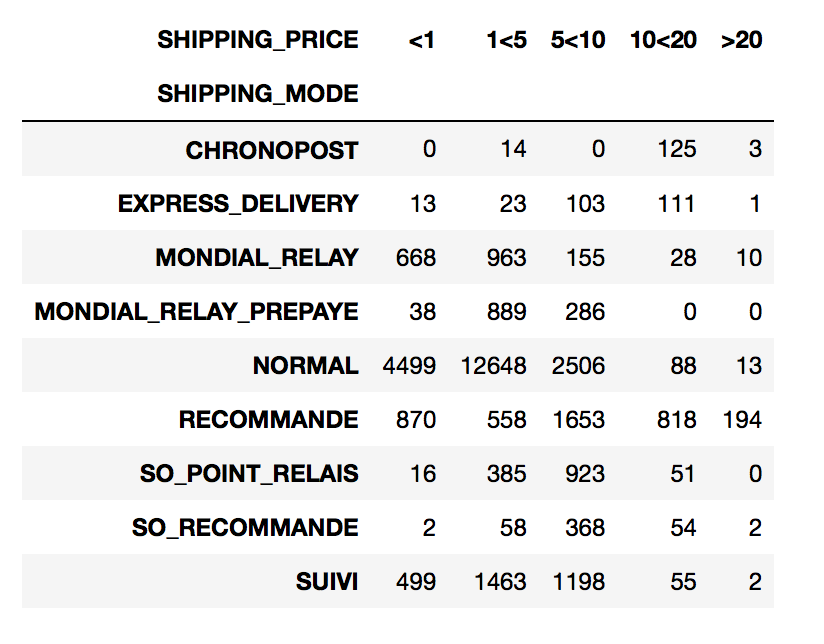
\includegraphics[scale=0.5]{assets/shipping} 
\end{center}

De plus, il y a une corrélation claire entre SHIPPING_MODE et SHIPPING_PRICE. Par exemple,
un SHIPPING_PRICE de plus de 20 a de grandes chance d'être de type RECOMMANDE.

\textbf{WARRANTIES_FLG et WARRANTIES_PRICE :}

Les personnes possédant une garantie sont plus susceptibles de porter des réclamations, en 
particulier de type WITHDRAWAL. Ceci est logique étant donné que le retrait peu être 
facilité par la prise d'une garantie.

Nous n'observons pas de corrélation claires entre le prix de la garantie et le type de
réclamation.

\textbf{PRICECLUB_STATUS :}

Cette variable est liée au nombre de points accumulé en effectuant des actions telles que
vendre des produits, parrainer un ami ou encore utiliser l'application PrimeMinister.
Avec ces points l'utilisateur peut occasionnellement bénéficier d'offres et de réductions.

Il n'y a pas de lien clair entre PRICECLUB_STATUS et les réclamations.

\textbf{REGISTRATION_DATE et PURCHASE_COUNT :}

\begin{center}
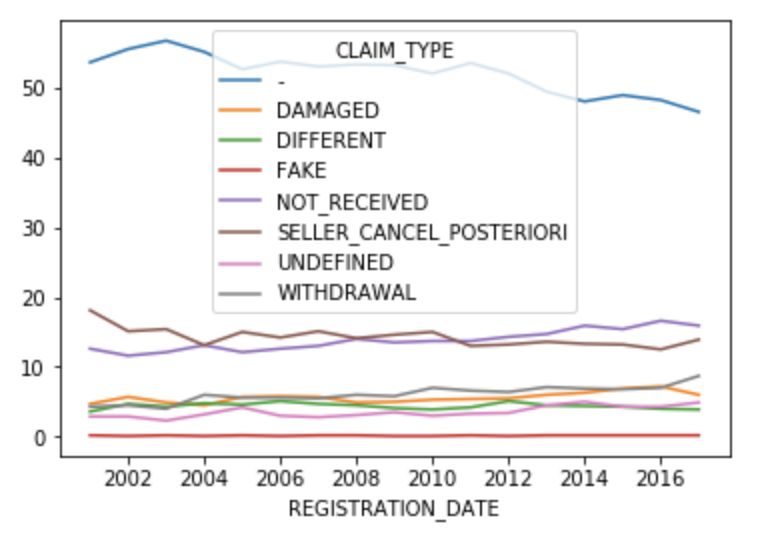
\includegraphics[scale=0.5]{assets/registrationdate} 
\end{center}

Nous observons que les récents utilisateurs ont plus tendance à porter de réclamations.
Il est notable que les acheteurs avec de l'expérience sur le site sont moins susceptibles
de porter des réclamations WITHDRAWAL et UNDEFINED. Cela fait sens car un utilisateur 
habitué a moins de chance de s'être trompé dans sa commande et de la retirer.
Cependant ces acheteurs ont aussi moins tendance a ne pas recevoir leur colis ou à recevoir  
un colis endommagé. Ceci peut s'expliquer par les habitudes des consommateurs qui avec le 
temps n'achètent qu'auprès des vendeurs en qui ils ont confiance.

De manière prévisible, il y a une corrélation importante entre l'année d'inscription de
l'utilisateur et le nombre de commandes passées.

De plus, nous pouvons observer un fossé clair entre les utilisateurs très récents (<5 items 
achetés) et les autres. Pour cette raison il peut être intéressant de créer une variable
supplémentaire pour mettre en avant le fait qu'un utilisateur soit novice ou non.

\textbf{BUYER_BIRTHDAY_DATE :}

\begin{center}
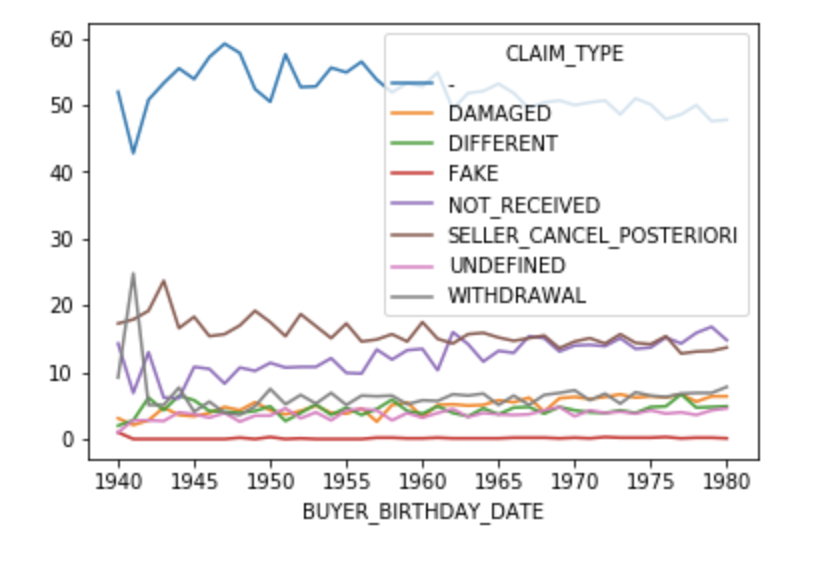
\includegraphics[scale=0.5]{assets/age} 
\end{center}

Une corrélation peu évidente peut être observée entre l'âge et les réclamations. 
En effet, les individus plus jeunes ont probabilité légèrement plus grande que la moyenne
de porter un réclamation de type NOT_RECEIVED.

\textbf{BUYER_DEPARTMENT, SELLER_DEPARTMENT et SELLER_COUNTRY:}

Pour observer plus facilement l'influence de la localisation des acheteurs et vendeurs
nous avons crées une variable supplémentaire permettant d'identifier utilisateurs par leur
région au lieu de leur département. 

Il n'y a pas cependant pas d'influence visible entre la région de l'acheteur et le type de
réclamation si l'acheteur vit en France. Nous pouvons seulement noter qu'en Ile de France
et dans la région PACA les colis sont légèrement plus susceptibles de ne pas arrivés
à destination.

Bien entendu, nous pouvons observé que les colis venant de l'étranger sont plus sujets à 
réclamation. Il peut donc être intéressant de créer une variable binaire supplémentaire 
pour mettre l'accent sur le fait que le colis vienne de l'étranger ou non.

On peut noter cependant que certains pays européens ont des taux de réclamations 
proches de la moyenne voir meilleurs (GERMANY : 39,1\%, BELGIUM : 41,8\%, LUXEMBOURG : 41,5\%),
alors que pour les colis provenant d'autres pays européens proches ont un taux de réclamations pour colis 
non reçu beaucoup plus élevé que la moyenne (19,2\% pour UNITED KINGDOM). 
Il semble donc difficile de regrouper ces pays en catégories et il sera nécessaire de créer
une indicatrice pour chacun de ces pays lors de la phase de feature engineering.

\textbf{BUYING_DATE :}

Cette variable est codé au format 'MM/AAAA' dont nous extrayons uniquement le mois qui est ici 
l'élément qui nous intéressent car toutes les ventes sont réalisées sur l'année 2017.

Nous remarquons d'ailleurs que les données s'arrête au mois d'octobre, ce qui est regrettable
puisque la période de Noël, particulièrement prolifique pour les sites de e-commerce, n'est 
pas représentée. Il aurait été intéressant de visualiser l'impact de cette période sur les
réclamations.

Dans ce jeu de données, le mois de Janvier est celui où le plus de commande sont réalisées,
et c'est aussi le mois où le plus de réclamations sont faites. De même, le mois d'Octobre
est le plus calme en terme de ventes mais aussi en terme de pourcentage de réclamations
faites. La tendance est donc que plus il y a de flux de commandes plus il risque d'y avoir
des réclamations.

\textbf{SELLER_SCORE_COUNT et SELLER_SCORE_AVERAGE :}

Logiquement, nous observons que le nombre de produits vendus par le vendeur est négativement
corrélé avec le taux de réclamations portées. De même, les vendeurs avec les meilleurs
notes moyennes sont les plus fiables. En particulier, les vendeurs avec une note moyenne de
49/50 sont peu nombreux (3994) et au dessus du lot en terme de fiabilité (seulement 12,4\%
de réclamations). Il peut donc être interessant de leur attribuer une variable binaire pour 
renforcer cet écart de fiabilité.

Cependant, il faut de noter que très petits nombre de vendeurs (51) ont une note moyenne 
maximale de 50/50 et ont cependant un taux de réclamation moyen très élevé (72,5\%).
Ces vendeurs sont peu être des comptes fake qui ont réussis à obtenir la note maximale
pour attirer des clients ou bien des anomalies. Dans tous les cas, il ne faut pas les 
classer parmi les bon vendeurs. Il ne faut pas non plus les considérer comme des outliers
et les retirer du jeu de données car le taux de réclamation qui est lié à ces vendeurs est 
significatif et peut contribuer à améliorer notre prédicteur.

\begin{center}
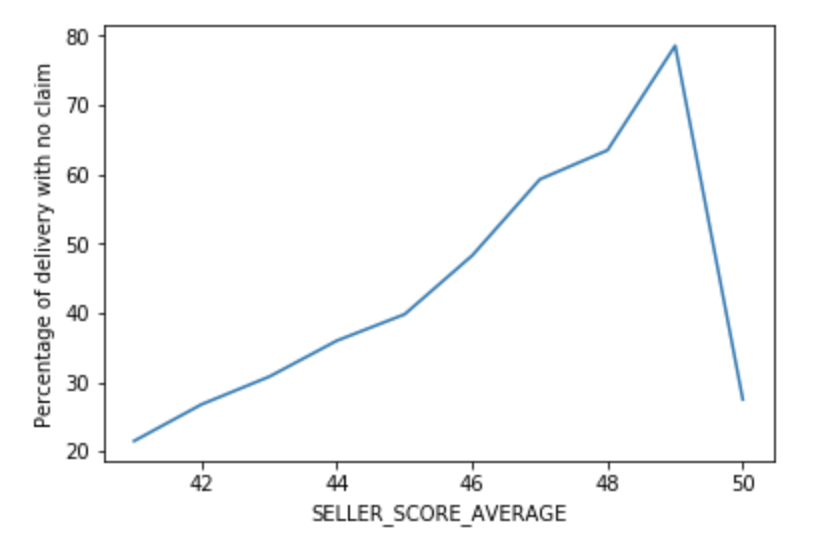
\includegraphics[scale=0.5]{assets/sellerscore} 
\end{center}

Nous observons de plus une corrélation importante et prévisible entre SELLER_SCORE_COUNT et 
SELLER_SCORE_AVERAGE.

\textbf{PRODUCT_TYPE et PRODUCT_FAMILY :}

Nous remarquons que les produits appartenant à la famille ELECTRONICS ont le taux le plus 
élevé de réclamations DAMAGED (10,8\% contre 5,1\% en moyenne). En effet les produits
électroniques tels qu'une télévision sont plus fragiles et susceptibles d'être 
endommagé lors du transport.


\textbf{ITEM_PRICE :}

Les produits les moins cher sont moins susceptible de mener à une réclamation.
En particulier les réclamations pour FAKE sont quasiment toujours des produits peu chers.
De même ce sont surtout les achats peu chers qui risque de ne pas arriver à destination.
Les produits couteux ont en revanche plus de chance de mener à un retrait de commande.

Les produits dont le prix est compris dans l'intervalle 100<500 ont typiquement plus de
chance d'arriver endommagé. Cela correspond au prix des appareils électroniques qui comme
nous l'avons observé précédemment sont plus souvent endommagé lors du transport.





























\chapter{Feature Engineering}

Cette section présente les principales transformations du jeu de données mises en oeuvre.
Cela comprend en particulier la transformation des variables catégorielles en
indicatrices ou dummy variables (SHIPPING_MODE, PRODUCT_FAMILY,...), le mapping des variables 
ordinales en variables d'entiers (SHIPPING_PRICE, PURCHASE_COUNT, ...),
compléter les valeurs manquantes et enfin créer de nouvelles variables.

\textbf{Variables transformées :}

\begin{itemize}
\item REGISTRATION_DATE est transformée en BUYER_SENIORITY indiquant le nombre d'années
d'ancienneté de l'utilisateur sur le site plutôt qu'une année 
\item BUYER_BIRTHDAY_DATE est remplacée par BUYER_AGE pour la même raison
\end{itemize}

\textbf{Variables créées :}

\begin{itemize}
\item UNEXPERIENCED_BUYER pour les individus qui ont effectué moins de 5 achats sur le site
\item VIP_SELLER pour les vendeurs ayant une note de 49/50
\item BUYER_REGION et SELLER_REGION représentant les régions des vendeurs et acheteurs.
Cette variables vient renforcer les variables BUYER_DEPARTMENT et SELLER_DEPARTMENT.
\item BUYER_IS_ABROAD et SELLER_IS_ABROAD indiquant que le vendeur/acheteur est à l'étranger.
\item SAME_REGION_BUYER_SELLER et SAME_DEPARTMENT_BUYER_SELLER pour indiquer si l'acheteur
et le vendeur d'une commande sont issus da la même région ou du même département.
\item SELLER_BUYER_REGION_DISTANCE distance en kms entre la ville principale de la région
du vendeur et la ville principale de la région de l'acheteur. Cette variable, obtenue en 
réalisant une matrice de distance relatives entre chaque région permet d'apporter une
information supplémentaire quant à la distance approximativement parcourue lors de la 
livraison lorsque le vendeur et l'acheteur sont en France. 
\item SELLER_COUNTRY_DISTANCE indiquant la distance relative entre le pays du vendeur et la France. 
Cette distance est échelonnée suivant une échelle de 0 à 4, 0 étant pour FRANCE METROPOLITAINE et 4 pour les 
pays les plus éloignées tels que JAPON, AUSTRALIE. Cette variable vient donc prolonger la variable
SELLER_BUYER_REGION_DISTANCE lorsque le vendeur est à l'étranger.
\end{itemize}

\textbf{Remplacement des valeurs manquantes :}

\begin{itemize}
\item  BUYER_AGE : méthode ffill
\item WARRANTIES_PRICE : les valeurs manquantes correspondent au cas où l'utilisateur n'a 
pas pris de garantie (même quantité de valeurs manquantes qu'il n'y a de False dans la 
variable WARRANTIES_FLG) et sont donc mises à 0.
\item  SHIPPING_PRICE : nous avons considéré que les valeurs nulles correspondent au cas
où les frais de livraisons sont gratuits et donc mis ces valeurs à 0
\end{itemize}

\textbf{Cas particulier :}

PRICECLUB_STATUS peut être vu comme une variable catégorielle nominale et être transformée
en variables binaires. Cependant, il y a une hiérarchie entre les différents 
status : UNSUBSCRIBED < REGULAR < PLATINUM < SILVER < GOLD. Nous avons donc préféré transformer
cette variable en une variables d'entiers (0 pour UNSUBSCRIBED jusqu'à 4 pour GOLD).






\chapter{Prédicteurs et résultats}

\section{Comparaison des modèles mis en place}

Les modèles présentés ci-dessous ont été testés en cross validation avec des
paramètres par défaut parmi les algorithmes suivants : Random Forest, Gradient Boosting 
avec XGBoost, Multilayer Perceptron, KNN.
Si les performances en cross validation étaient similaires entre les différents algorithmes
testés, nous utilisions alors un GridSearchCV pour optimiser les paramètres des modèles et
déterminer le meilleur. 
Si au contraire un modèle était d'emblée au dessus des autres en termes de performances, 
seul cet algorithme était alors optimisé avec GridSearchCV.

\textbf{1-} Le premier modèle mis en place avait pour but d'éviter la surcharge de variables et de 
synthétiser l'information dans des variables plus parcimonieuses. C'est dans ce but que les 
variables BUYER_REGION et SELLER_REGION ont été créées à la place de BUYER_DEPARTMENT et
SELLER_DEPARTMENT. Par exemple, la variable BUYING_DATE avait été synthétisée en seulement
3 groupes significatifs représentant les 3 périodes de l'année où les pourcentages de 
réclamations et le nombre de ces réclamations étaient similaires. De même, la variable
PRODUCT_TYPE qui possède 137 niveau n'avait été restreinte qu'aux types ayant un impact visible
sur le type de réclamation. 

AUC : 0,57
algorithme : random forest (n_estimators=100).

\textbf{2-} Le deuxième modèle mis en place a consisté cette fois-ci à garder le plus d'information
possible quitte à risquer d'avoir un peu de sur-apprentissage. Nous avons ainsi à la fois 
gardé les informations liées aux départements mais aussi celles liées aux régions et 
transformé l'ensemble des niveaux de la variable PRODUCT_TYPE en variables binaires.

AUC : 0,60
algorithme : random forest (n_estimators=100)

\begin{center}
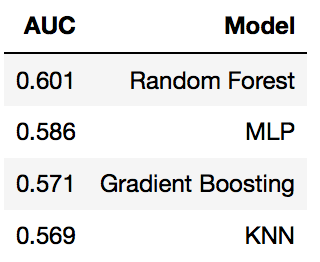
\includegraphics[scale=0.5]{assets/auc1} 
\end{center}

\textbf{3-} L'avancée majeure de notre modèle vient avec cette troisième phase où nous avons
tenter de prédire dans un premier temps la présence ou l'absence de réclamation et le cas 
échéant, prédire le type de réclamation avec un second modèle entrainé uniquement sur les
données où une réclamation a été portée. Les variables restent les mêmes qu'au modèle
précédent. La motivation derrière ce changement est que la classe '-' représente 50\%
de l'effectif total et correspond aussi au cas singulier de l'absence de réclamation, 
alors que les autres labels correspondent à un type de réclamation.
C'est avec cette amélioration que nous nous sommes hissés dans le top 10 du classement.

AUC : 0,63
algorithme de prédiction claim/no claim : random forest (n_estimators=200).
algorithme de prédiction du type de claim : random forest (n_estimators=100).

\textbf{4-} Une étape importante a ensuite été de modifier l'encodage du vecteur des
réclamations qui était à présent encodé avec un labelBinarizer qui est typiquement utilisé
dans les problèmes de classification multiclasses pour obtenir des variables binaires.
Nous avons utilisé ici un encodage différent en associant un entier à chaque type de
réclamation, classés par ordre de fréquence d'apparition dans le jeu de donné : 0 lorsqu'il
n'y a pas de réclamation jusqu'à 7 pour FAKE. Cet encodage a apporté un gain non négligeable
dans notre score avec les mêmes algorithmes.

AUC : 0,64
algorithme de prédiction claim/no claim : random forest (n_estimators=200).
algorithme de prédiction du type de claim : random forest (n_estimators=100).

\begin{center}
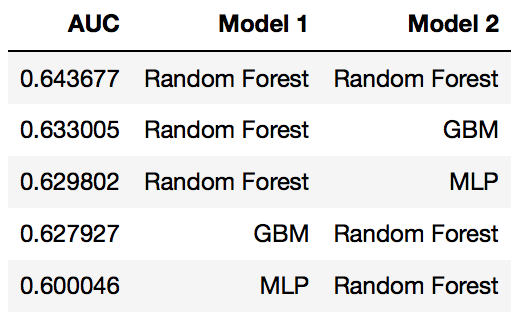
\includegraphics[scale=0.5]{assets/auc2} 
\end{center}

\textbf{5-} Les dernières modifications apportées à notre modèle résident dans la création
des features liés aux distances relatives entre acheteur et vendeur SELLER_BUYER_REGION_DISTANCE 
et SELLER_COUNTRY_DISTANCE. 

AUC : 0,649
algorithme de prédiction claim/no claim : random forest (n_estimators=200).
algorithme de prédiction du type de claim : random forest (n_estimators=100).

Avec cette dernière modification nous avons alors atteint la 2nde place du classement,
le premier groupe ayant un score de 0,650 à cet instant.

\section{Analyse des résultats}

Nous pouvons noter que l'algorithme de random forest s'est toujours avéré le plus efficace
dans tous les types de modèles testés.

Parmi les paramètres testés avec GridSearchCV seul le paramètre n_estimators semble 
déterminant pour notre problème, les autres paramètres étant systématiquement optimisés
avec leur valeur par défaut :

\begin{itemize}
\item max_features='auto'
\item criterion='Gini'
\item max_depth=None
\end{itemize}

Un des changement déterminant dans l'amélioration de notre score a été le passage d'un
modèle de prédiction simple à un modèle en deux temps, avec un premier algorithme
de classification binaire claim/no claim. Nous pouvons observer avec les matrices de confusion
ci-dessous la différence majeure qui réside dans ce changement de méthode.

\vspace{0.5cm}
\textbf{Matrice de confusion du modèle 2:}
\vspace{0.5cm}
\begin{center}
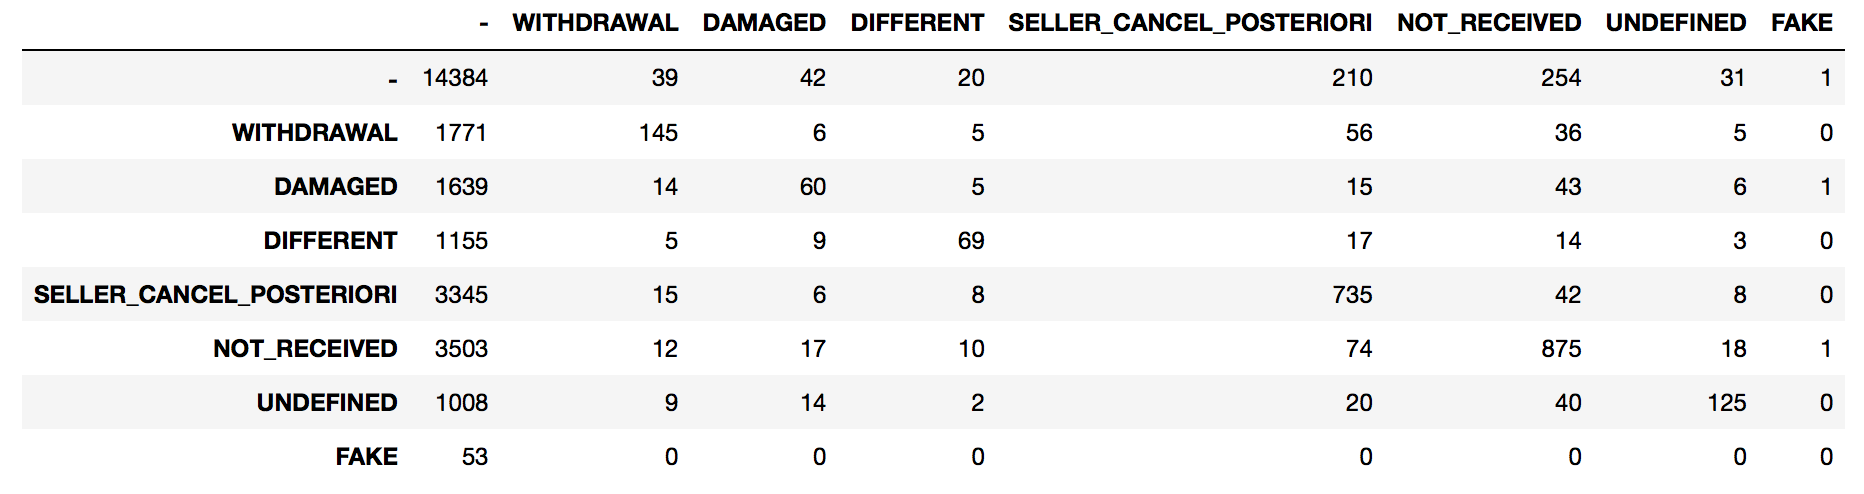
\includegraphics[scale=0.5]{assets/confmat1} 
\end{center}
\vspace{1.5cm}

\textbf{Matrice de confusion du modèle 3:}
\vspace{0.5cm}
\begin{center}
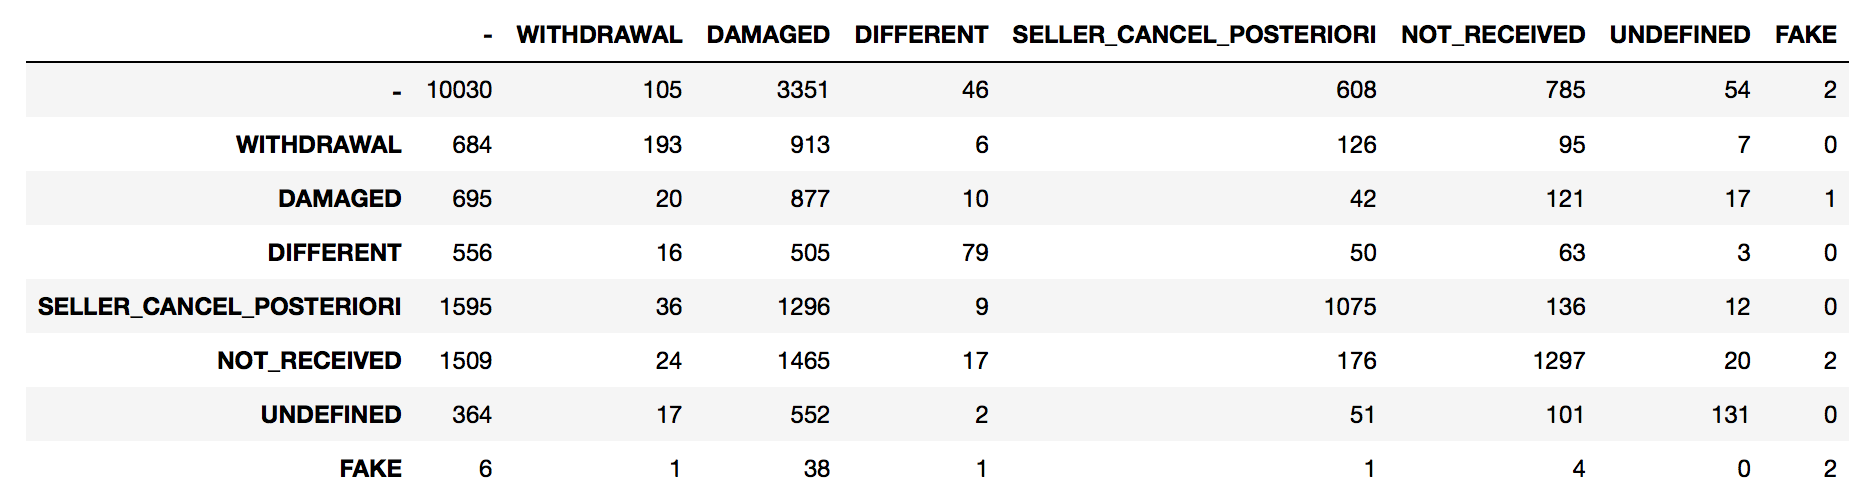
\includegraphics[scale=0.5]{assets/confmat2} 
\end{center}
\vspace{0.5cm}

En effet ce changement réside dans le fait que le modèle 2 a plus tendance a prédire qu'il
n'y aura pas de réclamation (biais conservateur) alors que le modèle 3 au contraire est plus 
susceptible de prédire qu'il y a réclamation (biais libéral). Le modèle 2 prédit 
majoritairement '-' qui est la classe majoritaire mais reste tout de même performant
sur les autres classes. En effet, en dehors des prédictions '-' le modèle 2 prédit 
majoritairement les bons types de réclamations. Cependant, le modèle 3 qui "prend plus de 
risque" est plus performant car il prédit mieux chacun des types de réclamations.



\chapter{Conclusion}

Ce projet nous a permis de mettre en pratique nos acquis en machine learning et en data 
science en nous confrontant a un problème issu de l'industrie. Nous avons notamment réalisé
au cours de cette étude toute l'importance du feature engineering. L'ajout d'une seule variable
peut s'avérer déterminante, comme cela a été le cas avec les derniers features de comparaison
des distances entre acheteurs et vendeurs. Cette étape est aussi celle qui demande le plus
de temps et d'effort et ne doit pas être bâclée en se contentant de
transformer les variables catégorielles du jeu de données en variables binaires. De plus,
nous avons pu nous rendre compte que l'intuition et l'expérimentation est aussi 
essentielle en machine learning. Beaucoup d'idées peuvent sembler bonnes et suivre une
certaine logique mais il faut avant tout tester ces idées pour voir émerger un modèle
efficace. C'est dans cette démarche que nous avons pu constater l'efficacité de passer
sur un modèle de prédiction en deux temps.

Pour améliorer notre modèle nous aurions pu pousser plus loin l'étude des distance entre
vendeurs en acheteurs en calculant les distance entre départements plutôt qu'entre région.
Dans ce but nous avons tenté d'exploiter l'API google maps pour créer cette matrice de distances de taille
96x96 mais la limite de requêtes imposée par l'API sans clé d'accès payante ne permet pas 
le téléchargement complet des données. 
Nous aurions pu aussi tenter de mettre en place une méthode plus avancée telle que le 
stacking qui est souvent utilisée pour gagner les challenges de data science. Cependant,
la deuxième place que nous occupons à l'heure actuelle est très encourageante.


%% insert a Python code block
%\begin{codeblock}
%print("Hello World !")
%\end{codeblock}

%% use the \tcode command to insert inline code
%The previous code prints \tcode{"Hello World !"}.

%\begin{center}
%  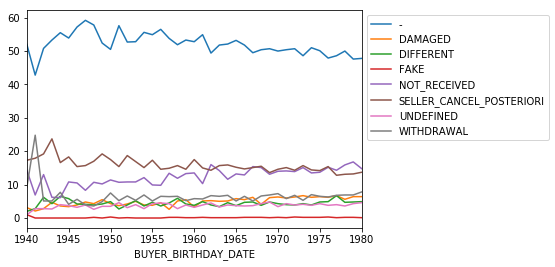
\includegraphics[scale=0.75]{assets/buyer-birthday-date-claim-percentage-crosstab}
%\end{center}


\begin{appendices}
%% Put appendices here
\end{appendices}


\backmatter

\printindex

\newpage

\renewcommand{\leftmark}{Bibliographie}
\bibliography{bib} 
\bibliographystyle{abbrv}




\end{document}
